\documentclass[class=minimal,border=2pt]{standalone}

\usepackage{tikz}
\usetikzlibrary{shapes,arrows}
\usepackage{verbatim}
\usepackage{pgfplots, pgfplotstable}
\begin{document}
	
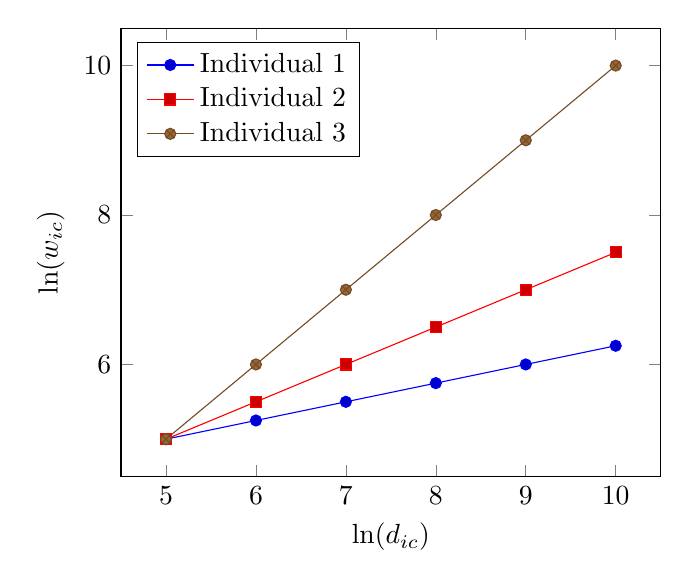
\begin{tikzpicture}
   \begin{axis}[
     xlabel = $\ln(d_{ic})$,
     ylabel = $\ln(w_{ic})$,
     legend pos = north west,
     ymin = 4.5,
     ymax = 10.5
     ]
     \addplot coordinates {
       (5, 5)
       (6, 5.25)
       (7, 5.5)
       (8, 5.75)
       (9, 6)
       (10, 6.25)
     };
     \addlegendentry{Individual 1}
     \addplot coordinates {
       (5, 5)
       (6, 5.5)
       (7, 6)
       (8, 6.5)
       (9, 7)
       (10,7.5)
     };
     \addlegendentry{Individual 2}
     \addplot coordinates {
       (5, 5)
       (6, 6)
       (7, 7)
       (8, 8)
       (9, 9)
       (10, 10)
     };
     \addlegendentry{Individual 3}
  \end{axis}
\end{tikzpicture}
\end{document}